\chapter{背侧前额叶皮层:基于最近事件生成目标}
背侧PF皮层有助于根据顺序、时间和空间环境生成目标,它的连接解释了为什么只有它才能做到这一点。背侧PF皮层,包括中外侧PF皮层(46区),通过与后顶叶皮层、前运动皮层和PF皮层的其他部分连接来发挥作用。顶叶连接提供了许多用于生成目标的空间和时间背景。与运动前区域的联系导致这些目标的实现,通常是通过手的运动。与眶侧PF皮层的连接使背侧PF皮层能够根据单个事件预测目标选择的具体结果。背侧PF皮层位于背侧视觉流的末端,因此它可以规划目标序列,它可以具体或抽象地指定这些目标。在产生目标后,背侧PF皮层可以前瞻性地编码它们,直到行动的时候到来。鉴于背侧PF皮层在类人猿灵长类动物中进化(第2章),我们认为它在使用最近视觉事件的顺序、时间和位置来指导觅食选择和生成效率优化的目标序列方面具有优势。

\section{介绍}
第二章解释了灵长类动物的PF皮层在类人猿中随着新区域的出现而扩展。第三章涉及了其中的一些,例如极性PF皮层(10区),但在本章和下一章,它们是主要主题。由于类人猿依赖于白天漫长的觅食旅行,它们需要消耗大量的能量,并面临着很高的捕食风险。这种生活方式非常重视正确的觅食选择。在影响这种选择的因素中,视觉事件的位置、时间和顺序是突出的,因为类人猿利用了它们在中央凹和色彩视觉方面的进步。正如第二章所解释的,这些进步包括中央凹提供的精致的视觉敏锐度和三色视觉提供的增强的辨别能力。

这一章解释了觅食的选择部分取决于当前的环境,这是由选择时可用的刺激以及最近视觉事件的记忆所指定的。为了理解我们的意思,考虑一个简单的实验室任务:延迟匹配样本。猴子把一个刺激看作一个样本,然后看到一个或多个刺激需要选择。这种选择不仅取决于选择时的刺激,还取决于基于样本刺激的记忆。这两个因素共同构成了当前选择目标的背景。

由于记忆对当前情境起作用,这类实验的被试面临一个问题:最近发生了几件事,并选择了几个目标。本章的大部分内容探讨了背侧PF皮层如何帮助类人猿灵长类动物解决这个问题。许多文献都依赖于一个任务和一个区域:延迟反应任务,它依赖于中外侧PF皮层(46区)。因此,我们将讨论的重点放在第一章和第五章也提到的这个任务上。我们认为,因为受试者在这个任务中经历了一系列的视觉事件,并实现了一系列的目标,他们需要挑选出决定当前目标的事件。然后,我们回顾一系列其他任务,这些任务也要求主体在当前环境的基础上生成目标。
\section{区域}
在猕猴中,中外侧PF皮层位于主枕沟的吻侧三分之二(图6.1)。然而,它也延伸到这个沟的背侧和腹侧的凸面皮层。中外侧PF皮层(46区)有很多名字,有些很明确,有些则不太明确。
\begin{figure}
	\centering
	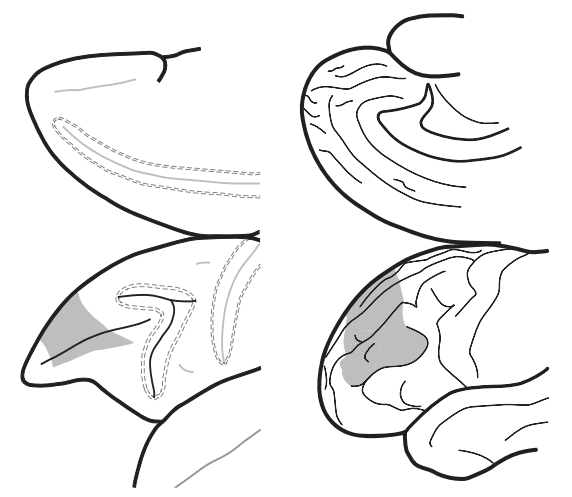
\includegraphics[width=0.7\linewidth]{image_pfc/Fig_6_1}
	\caption{猕猴(左)和人类(右)的背侧PF皮层。格式如图1.2所示}
	\label{fig:fig}
\end{figure}

Walker(1940)将沿主沟整个长度的皮层称为46区,但最近Petrides和Pandya(1999)将9/46区区分为该沟的尾端周围(见图1.2)。为了避免对46这个术语的不同用法的混淆,我们称沃克46区吻侧三分之二为中外侧PF皮层,尾侧三分之一为后外侧PF皮层。在人类中,这些分区位于额上回和额下沟之间。

尽管出现了这些新术语,但混淆的空间仍然很大。术语背侧前额叶皮层最初是指猴子的整个侧前额叶皮层(Pribram et al. 1952),但后来仅指主沟内和背侧的皮层(Mishkin et al. 1969)。在影像学文献中,指PF背外侧皮层已变得很常见,但该术语的使用通常非常松散,很少注意解剖标志。因此,我们在本书中避免使用这个术语。表1.2给出了我们所采用的术语。我们将PF背侧皮层包括主沟两岸的皮层和其背侧的凸面皮层(区域9),但不包括区域9的内侧部分。当然,这些划分并不是最终的结果,但它们在一定程度上反映了联系。
\section{定义和术语}


\section{指纹}

\subsection{损伤和激活}

\subsection{损伤和活动}

\subsection{活动和激活}




\subsection{结论}


